\subsection{Results & Analysis}

On our test set, across 10 different training sequences, we our bootstrapped trajectories
yieled an average success rate of 74\%. This represents a 15\% increase over the baseline 
approach which only used the initial human demonstrated trajectories. Our best performing
run gained an additional 10\% to reach an 84\% success rate overall. Fig.~\ref{fig:results} 
illustrates these results.

We believe that these results indicate the utility of this approach to improving
trajectory transfer with non-rigid registration. By successively warping from 
states that we have transferred trajectories successfully, we enable transfer
that penalizes less for deformations that preserve important aspects of the manipulation
task without hand-coding prior knowledge. For example, in our knot-tying task, trajectory 
will transfer robustly for deformations in the X-Y plane, but deformations in the Z dimension
will often cause unsucessful transfers. Fig.~\ref{fig:warps} illustrates this for one
example from our evaluation set. Directly warping with TPS-RPM fails because correspondences 
are hard to find. Even with correct correspondences, standard trajectory transfer is
prone to failure because the thin plate spline fit will penalize equally for all deformations.
By contrast, bootstrapping from successful trajectories discovers this structure
and is able to leverage it to succeed. 

We believe that these results indicate the utility of this approach. We have demonstrated that
given access to feedback about successful transfers can have large payoffs. However,
the particular algorithm we use to actually perform this bootstrapping exhibits large variance.
We believe that this can be combatted through more explicit and careful tradeoff between
exploration and exploitation. After the intial exploration phase, the focus on exploitation
can miss the potential to better transfer new trajectories. A more sophisticated treatement
of the exploration exploitation tradeoff in this setting is an important direction for future work.

\begin{figure}
  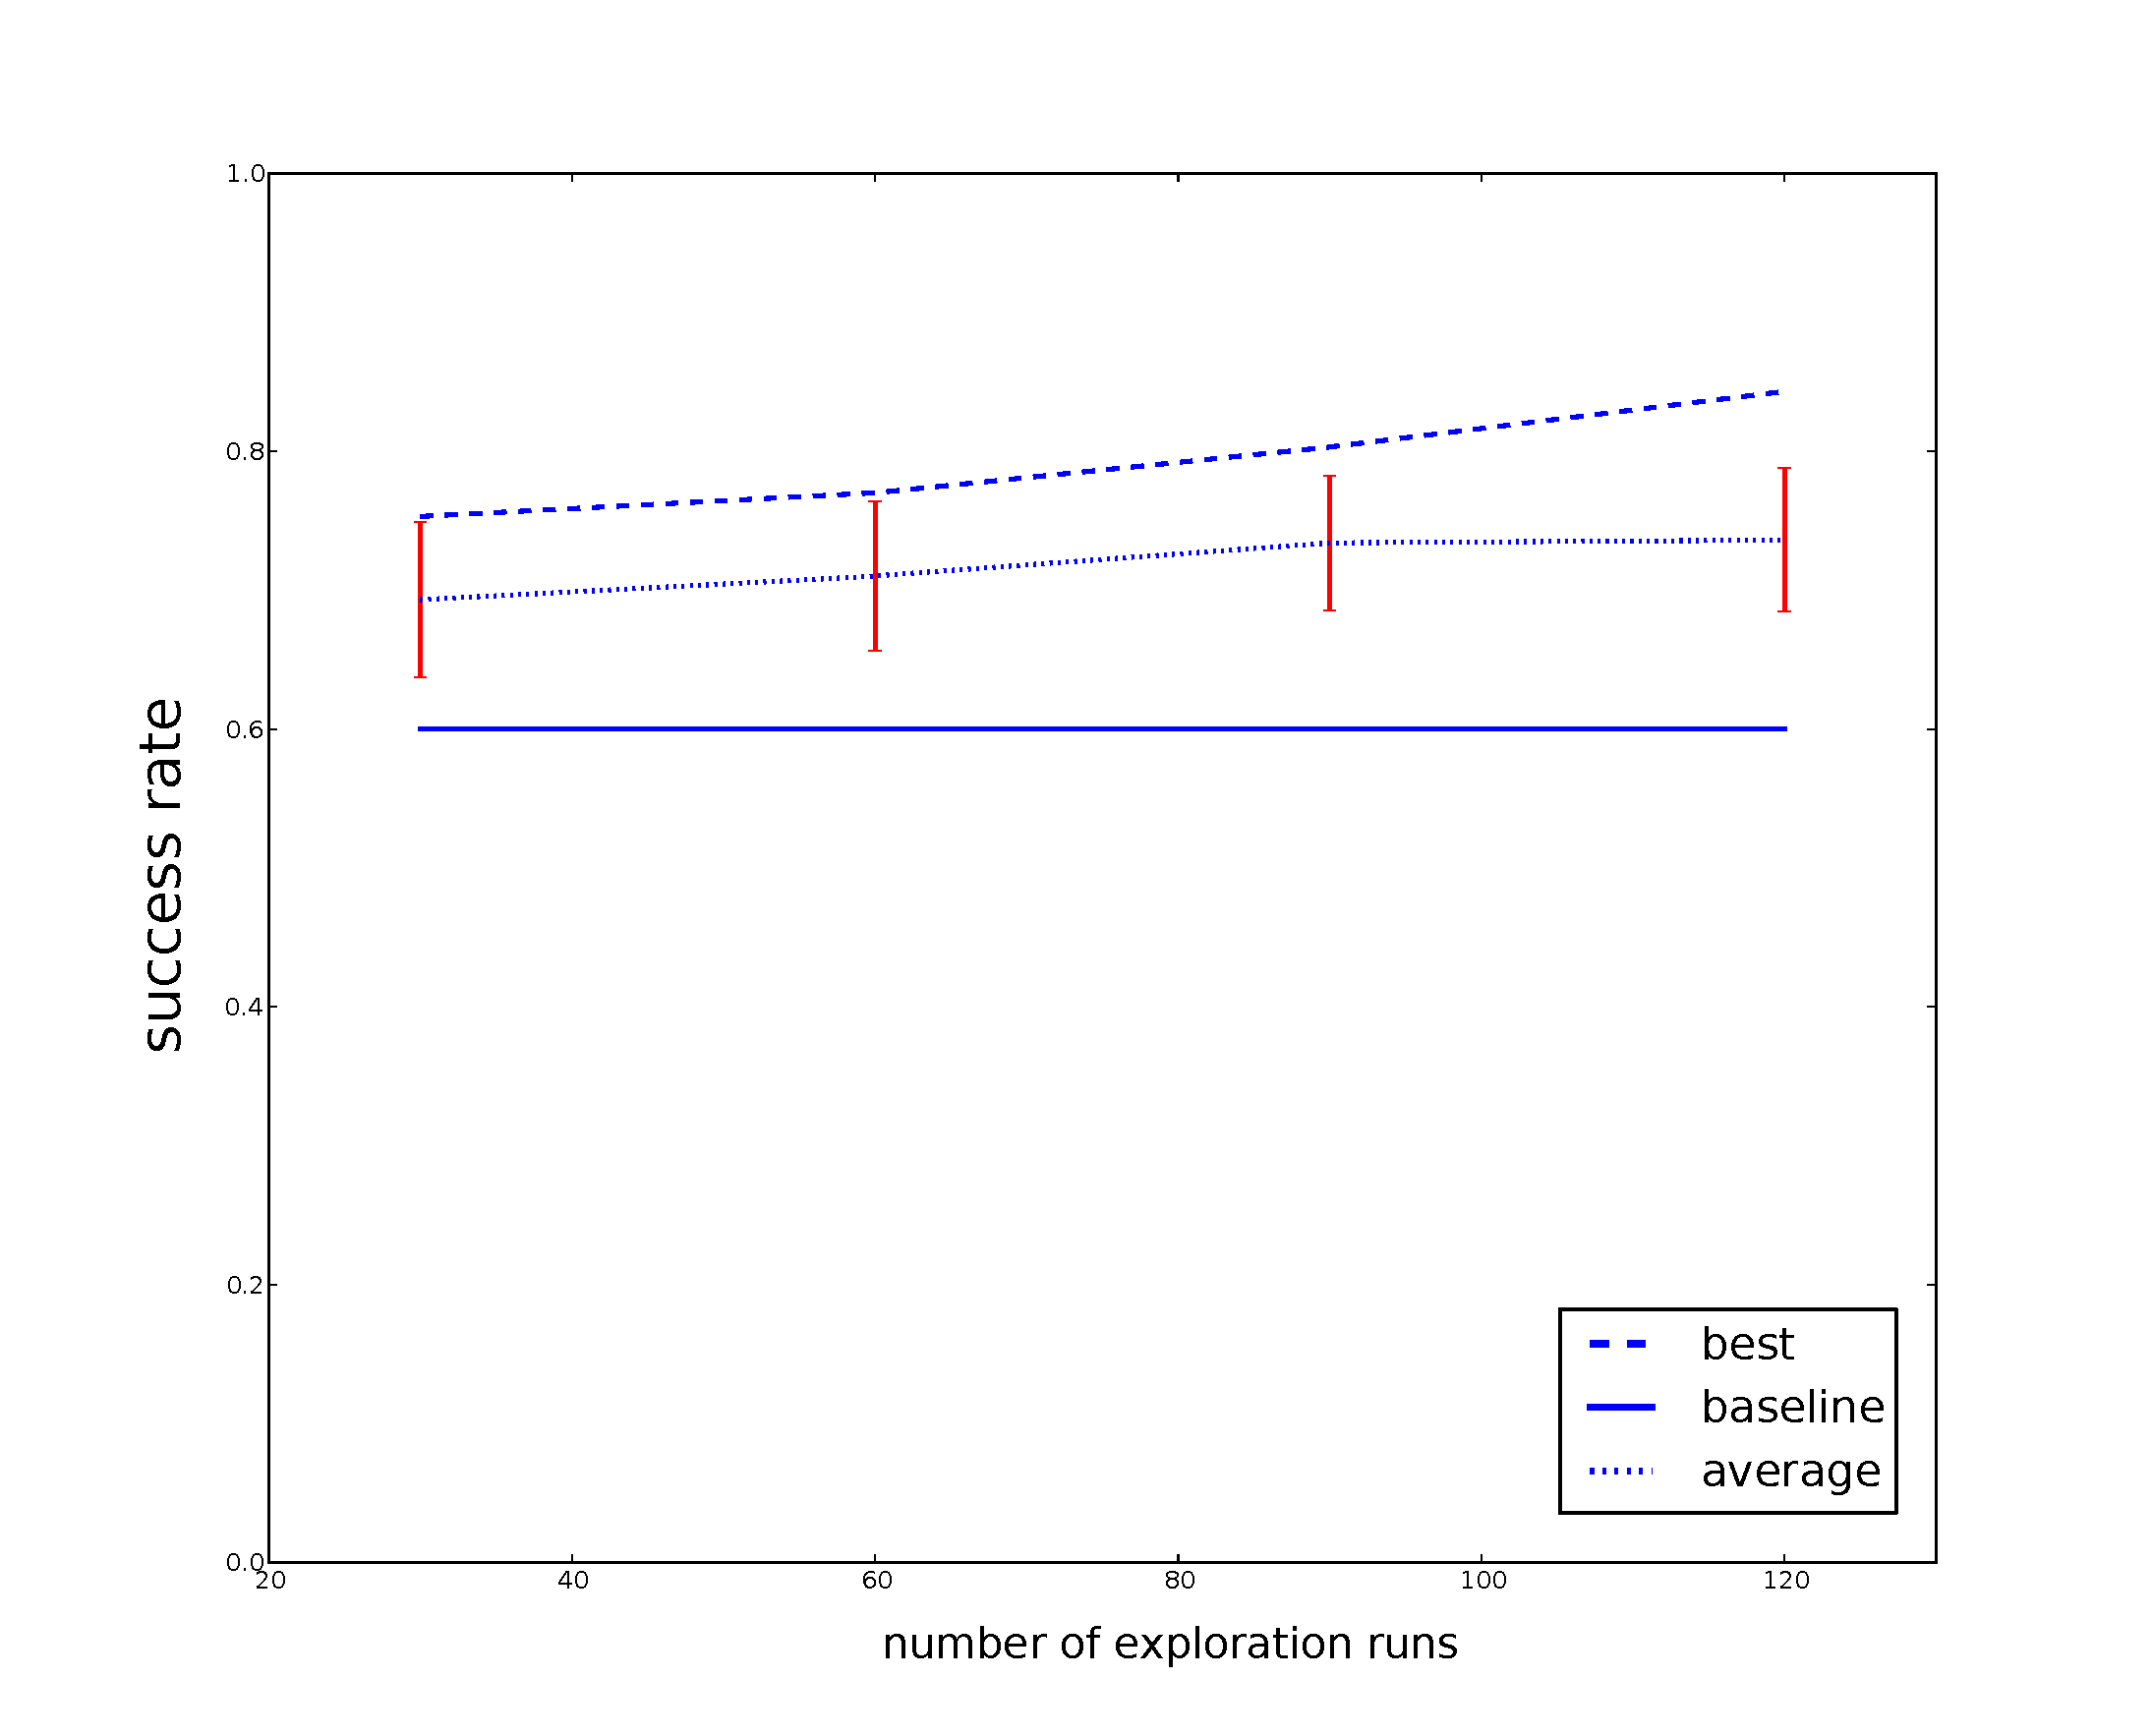
\includegraphics[width=\linewidth]{figs/results.pdf}
  \caption{Success rate of tying a an overhand knot in simulation with bootstrapped 
          examples compared with the baseline approach from Schulman et 
          al.~\cite{Schulmanetal_ISRR2013}. The problems for this scenario were generated
          by selecting a random initial state from a demonstration library and perturbed
          randomly by dragging random points on the rope. Directly transferring from the
          demonstrations achieves a success rate of 59\%. After doing 170 round of bootstrapping,
          we are able to improve on to an average of 74\% success. Our top performing trained set
          achieved 84\% success, an improvement of 25\% over the baseline. This success can
          be attributed to several factors, key among them are better modelling of states
          a trajectory can transfer to and ability to penalize less for deformations that 
          have allowed successful transfer in the past.}
  \label{fig:results}
\end{figure}

\begin{figure}
  \begin{subfigure}[b]{.48\linewidth}
    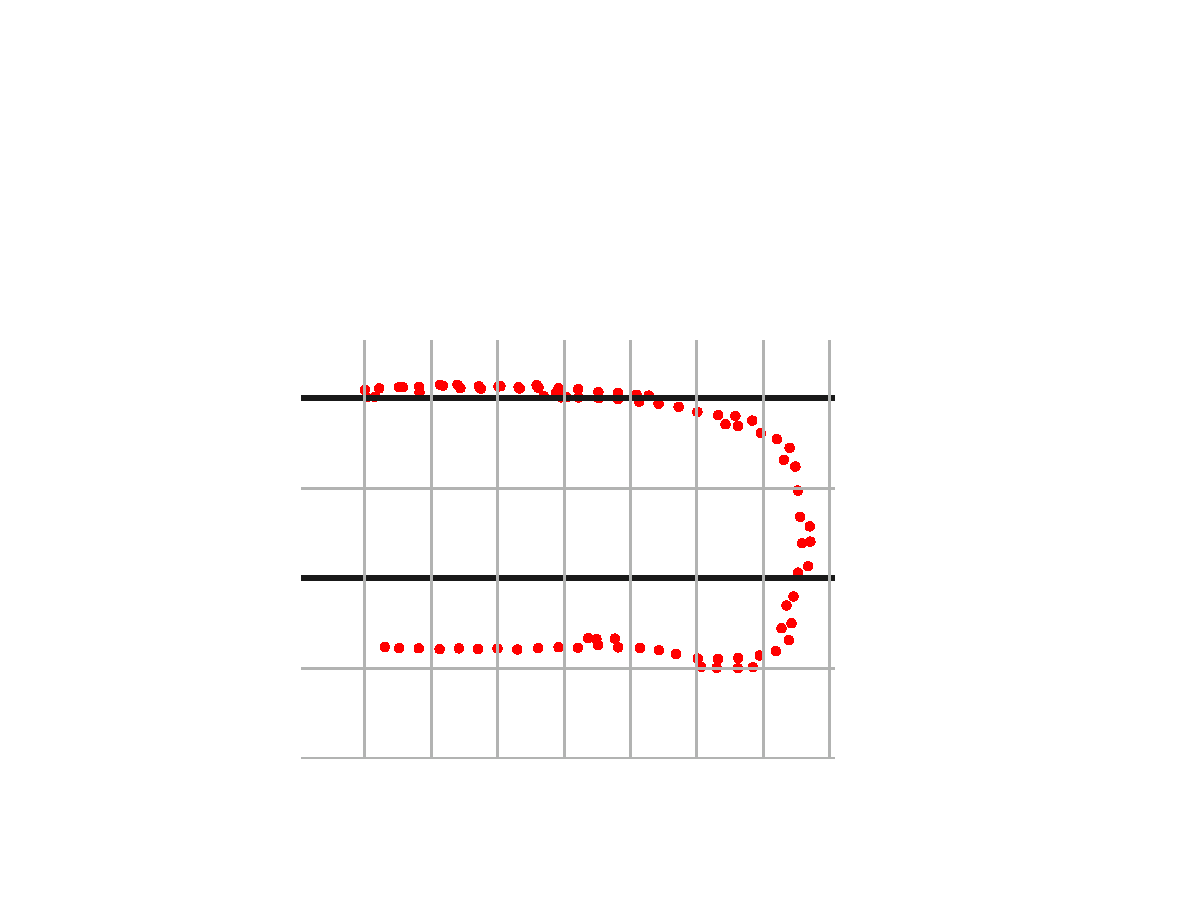
\includegraphics[width=\textwidth]{figs/orig.pdf}
    \caption{Original Segment}
    \label{fig:no_warp}
  \end{subfigure}
  \begin{subfigure}[b]{.48\linewidth}
    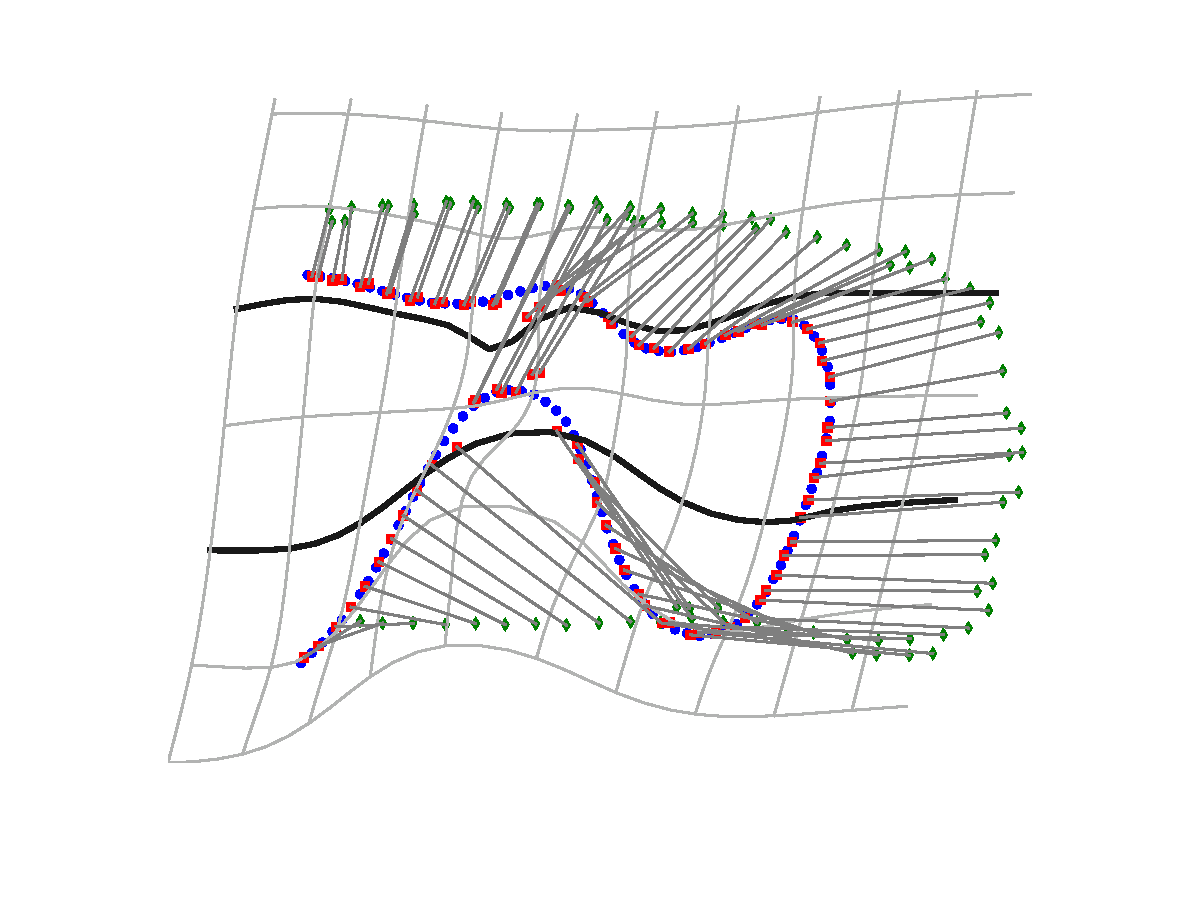
\includegraphics[width=\textwidth]{figs/warp_root.pdf}
    \caption{Directly Applying TPS-RPM}
    \label{fig:warp_root}
  \end{subfigure}
  \begin{subfigure}[b]{.48\linewidth}
    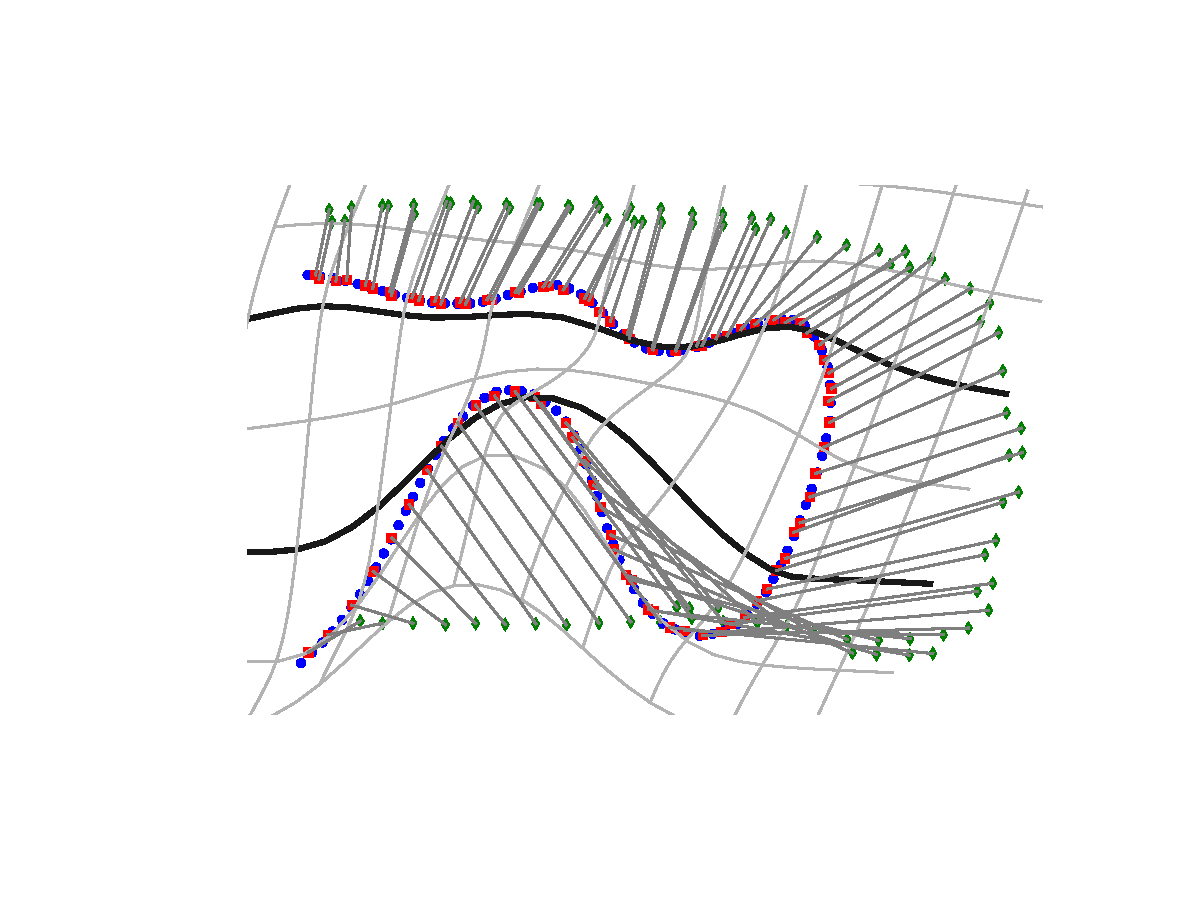
\includegraphics[width=\textwidth]{figs/warp_root_known.pdf}
    \caption{Known Correspondences}
    \label{fig:corresponds}
  \end{subfigure}
  \begin{subfigure}[b]{.48\linewidth}
    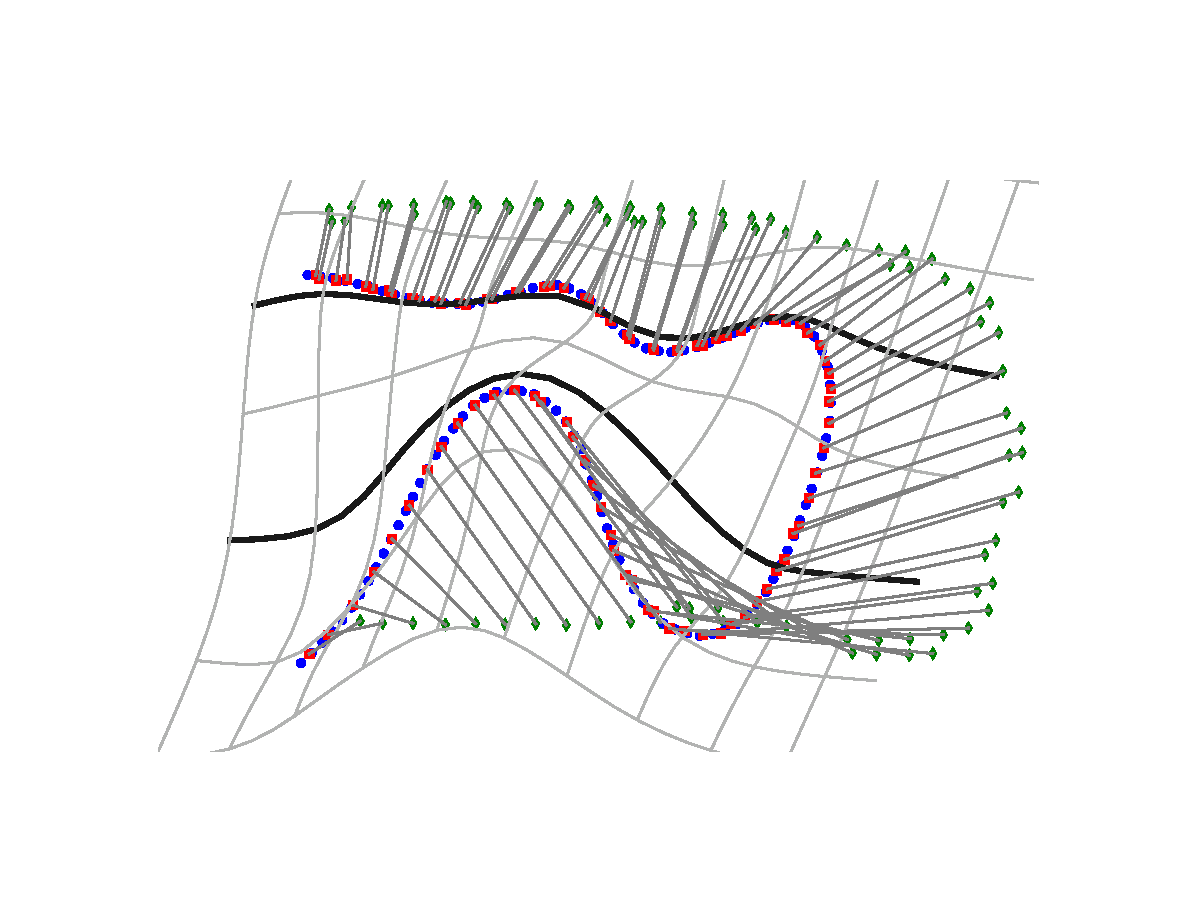
\includegraphics[width=\textwidth]{figs/warp_derived.pdf}
    \caption{Bootstrapping}
    \label{fig:bootstrap}
  \end{subfigure}
  \caption{Illustrations of various methods of Thin Plate Spline mappings.
  (a) shows the state from the demonstration being warped. (b) shows the results of directly warping from this state with TPS-RPM. The differences between the demonstration state and current state cause errors errors in the correspondences. (c) shows the results of directly fitting a thin plate spline with known correspondences. The intersection of the bold line and the rope (which are seperate in the initial scene) illustrates a large amount of non-rigidity in the $Z$-dimension to reduce the warping the X-Y plane. This can cause trajectory transfer to fail for this task. (d) shows the results of warping from a nearby bootstrapped state. The overall structure of the demonstration scene is better mapped into this scene because the iterated thin plate spline does not penalize for deformations that led to successful trajectory transfers during training.}
  \label{fig:warps}
\end{figure}

